\documentclass[a4paper,12pt]{scrartcl}
\usepackage[utf8]{inputenc}
\usepackage[ngerman]{babel}
\usepackage[T1]{fontenc}
\usepackage{amsmath}
\usepackage{stmaryrd}
\usepackage{wasysym}
\usepackage{lmodern}
\usepackage{graphicx}
\usepackage{paralist}
\usepackage{upgreek}
\usepackage{subfigure}
\usepackage{tipa}
\usepackage{amssymb}
\usepackage{gensymb}
\usepackage{dsfont}
\usepackage{mathtools}
\usepackage{ stmaryrd }
\usepackage{fancyhdr}
\usepackage{tikz}
\usetikzlibrary{arrows,automata}

%\title{Abgabe 1}
%\author{Rafael Heid, Julian Deinert, Sabrina Buczko Gruppe\\ 6 und 7}
%\date{Abgabe am 24.10.16}

\gdef\blatt{FGI-2 Aufgabenblatt 07}

\title{\blatt}
\date{Gruppe 07}
\author{Sabrina Buczko 6663234, Julian Deinert 6535880, Rafael Heid 6704828}


\pagestyle{fancy}
\fancyhf{}
\fancyhead[L]{\blatt}
\fancyhead[R]{Buczko, Deinert, Heid}
\fancyfoot[C]{\thepage}

\begin{document}
\maketitle
\newpage
\setcounter{section}{6}
% Section 7
\section{}
\setcounter{subsection}{2}
% Section 7.3
\subsection{}
% Section 7.3.1
\subsubsection{}
\begin{tikzpicture}[->,>=stealth',shorten >=1pt,auto,node distance=4cm, semithick]
  \tikzstyle{every state}=[fill=none,draw=none,text=black]

  \node[state] (A)              {$p2p4$};
  \node[state] (B) [right of=A] {$p1(2)p3(2)$};
  \node[state] (C) [below of=B] {$p1p3p4$};
  \node[state] (D) [right of=B] {$p1p2p3$};
  \node[state] (E) [below of=D] {$p2(2)$};
  \node[state] (F) [below of=A] {$p4(2)$};

  \path (A) edge              node {$t_3$} (B)
        (B) edge              node {$t_1$} (D)
            edge              node {$t_2$} (C)
        (D) edge              node {$t_1$} (E)
            edge [bend right] node [above] {$t_2$} (A)
        (C) edge              node {$t_1$} (A)
            edge              node {$t_2$} (F);
\end{tikzpicture}
% Section 7.3.2
\subsubsection{}
Eine Schaltfolge in der $t_3$ dreimal vorkommt und auf $t_3$ endet, ist besipielsweise:\\
\begin{math}
p2p4 \xrightarrow{t_3} 
p1(2)p3(2) \xrightarrow{t_1} 
p1p2p3 \xrightarrow{t_2} 
p2p4 \xrightarrow{t_3} 
p1(2)p3(2) \xrightarrow{t_1} 
p1p2p3 \xrightarrow{t_2} 
p2p4 \xrightarrow{t_3} 
p1(2)p3(2)
\end{math}
% Section 7.3.3
\subsubsection{}
\begin{itemize}
	\item{Lebendigkeit:}\\
		Das Netz ist nicht lebendig, da beispielswiese nach 
    dem Schalten von $t_3$, $t_2$ und wieder $t_2$ 
		die Markierung $p4(2)$ erreicht ist und von dort
    keine anderen Markierungen 
		mehr erreicht werden können.
	\item{Verklemmungsfreiheit:}\\
		Das Netz ist aus dem gleichen Grund wie für die 
		Lebendigkeit nicht verklemmungsfrei.
	\item{Reversibilität:}\\
		Das Netz ist aus dem bereits genannten Grund auch 
		nicht reversibel

\end{itemize}
% Section 7.3.4
\subsubsection{}
\begin{math}
  \begin{pmatrix}
  0\\
  1\\
  0\\
  1\\
  \end{pmatrix}
  \xrightarrow{t_3}
  \begin{pmatrix}
  2\\
  0\\
  2\\
  0\\
  \end{pmatrix}
  \xrightarrow{t_1}
  \begin{pmatrix}
  1\\
  1\\
  1\\
  0\\
  \end{pmatrix}
  \xrightarrow{t_2}
  \begin{pmatrix}
  0\\
  1\\
  0\\
  1\\
  \end{pmatrix}
  \xrightarrow{t_3}
  \begin{pmatrix}
  2\\
  0\\
  2\\
  0\\
  \end{pmatrix}
  \xrightarrow{t_1}
  \begin{pmatrix}
  1\\
  1\\
  1\\
  0\\
  \end{pmatrix}
  \xrightarrow{t_2}
  \begin{pmatrix}
  0\\
  1\\
  0\\
  1\\
  \end{pmatrix}
  \xrightarrow{t_3}
  \begin{pmatrix}
  2\\
  0\\
  2\\
  0\\
  \end{pmatrix}
\end{math}
% Section 7.3.5
\subsubsection{}
Wir verändern das Netz in folgenden Schritten:
\begin{enumerate}
  \item
  Wir löschen die Transistion $t_2$
  \item
  Wir biegen die Kante, die ursprünglich von $p1$ zu $t_2$
  führte, nach $t_1$ um. Da diese Kante bereits existiert,
  verleihen wir ihr ein Kantengewicht von $2$.
  \item 
  Wir biegen die Kante, die ursprünglich von $p3$ zu $t_2$
  führte, nach $t_1$ um. Da diese Kante bereits existiert,
  verleihen wir ihr ebenfalls ein Kantengewicht von $2$.
  \item
  Wir biegen schließlich die Kante, die ursprünglich von $t_2$ nach $p4$ führte, so um, dass sie nun von $t_1$ nach $p4$ führt.
\end{enumerate}
Nach diesen Schritten erhalten wir das folgende Netz:\\
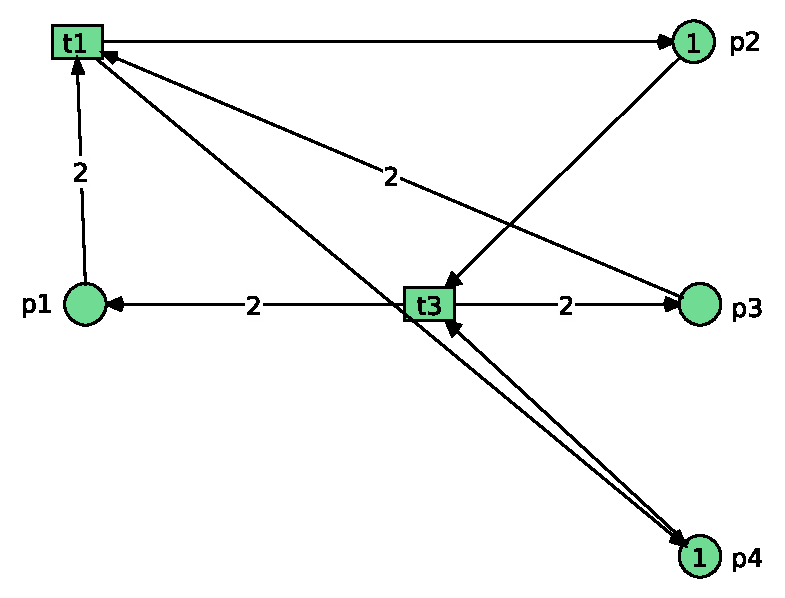
\includegraphics[scale=0.8]{G-6-A-07-Netz1-Buczko_Heid_Deinert.pdf}\\
Der Erreichbarkeitsgraph für diese Netz ist einfacher 
Strukturiert.\\
\begin{tikzpicture}[->,>=stealth',shorten >=1pt,auto,node distance=4cm, semithick]
  \tikzstyle{every state}=[fill=none,draw=none,text=black]

  \node[state] (A)              {$p2p4$};
  \node[state] (B) [right of=A] {$p1(2)p3(2)$};

  \path (A) edge              node {$t_3$} (B)
        (B) edge [bend right] node [above] {$t_1$} (A);
\end{tikzpicture}
\\
Aus dem Erreichbarkeitsgraph lässt sich erkennen, dass
das Netz nun nach dem initialen Schalten von $t_3$ durch 
schalten von $t_1$ immer wieder in den Ursprungszustand 
versetzt werden kann.
\begin{itemize}
  \item{Lebendigkeit:}\\
    Das Netz ist nun lebendig, da nur noch abwechselnd $t_3$ und $t_1$ geschaltet werden kann und sich das Netz nach jedem durchlauf dieser Schaltfolge wieder im Ursprungszustand $p2p4$ befindet.  
  \item{Verklemmungsfreiheit:}\\
    Das Netz ist aus dem gleichen Grund wie für die 
    Lebendigkeit nun auch verklemmungsfrei.
  \item{Reversibilität:}\\
    Das Netz ist aus dem selben Grund nun auch 
    reversibel

\end{itemize}
\end{document}